\documentclass[10pt]{beamer}

\usepackage[english]{babel}
\usepackage[utf8]{inputenc}
\usepackage{amsmath,amssymb,amsthm,latexsym}
\usepackage{mathrsfs}
\usepackage[all]{xypic}
\usepackage{tikz}
\usetikzlibrary{arrows,matrix}
\usepackage{eurosym}
\usepackage{listings}
\usepackage{textcomp}
\usepackage{soul}

\usepackage[bibstyle=beamer,citestyle=authoryear-comp,doi=false,isbn=false,eprint=false,maxnames=10]{biblatex}
\bibliography{defeo}
\usepackage{mysymbols}


\newenvironment{pictureframe}{
  \addtocounter{framenumber}{-1}
  \setbeamertemplate{navigation symbols}{}
  \setbeamercolor{background canvas}{bg=black}
  \begin{frame}[plain,fragile,environment=pictureframe]%
    \begin{center}%
    }{%
    \end{center}%
  \end{frame}%
}

\lstset{
  upquote=true,
  basicstyle=\ttfamily,          % print whole listing in typewriter
  keywordstyle=\color{blue}\bfseries, % bold blue keywords
  %identifierstyle=,           % nothing happens
  commentstyle=\color{green}, % green comments
  stringstyle=\color{red},      % typewriter type for strings
  showstringspaces=false     % no special string spaces
}

\usepackage[amssymb,amsfonts]{concmath}
\renewcommand{\sfdefault}{uop}
\mode<presentation>{%
  \usetheme{Boadilla}
  \usefonttheme[onlymath]{serif}
  \usecolortheme[rgb={0.56,0.3,0}]{structure}
  \setbeamercolor{alerted text}{fg=blue}
}
\renewcommand{\emph}[1]{{\usebeamercolor[fg]{structure}#1}}


\title{Transposition principle and applications}
\author[Luca De Feo]{Luca De Feo\\\small{joint work with É. Schost and M. Boespflug}}
\institute{IRMAR}
\date{Rennes, April 1, 2011}


\begin{document}

\begin{frame}
  \titlepage
\end{frame}

%%
%%

\begin{frame}
  \frametitle{Or, ``The day I discovered I suffer from schizophrenia''}

  \begin{columns}[c]
    \begin{column}{0.5\textwidth}
      \begin{center}
        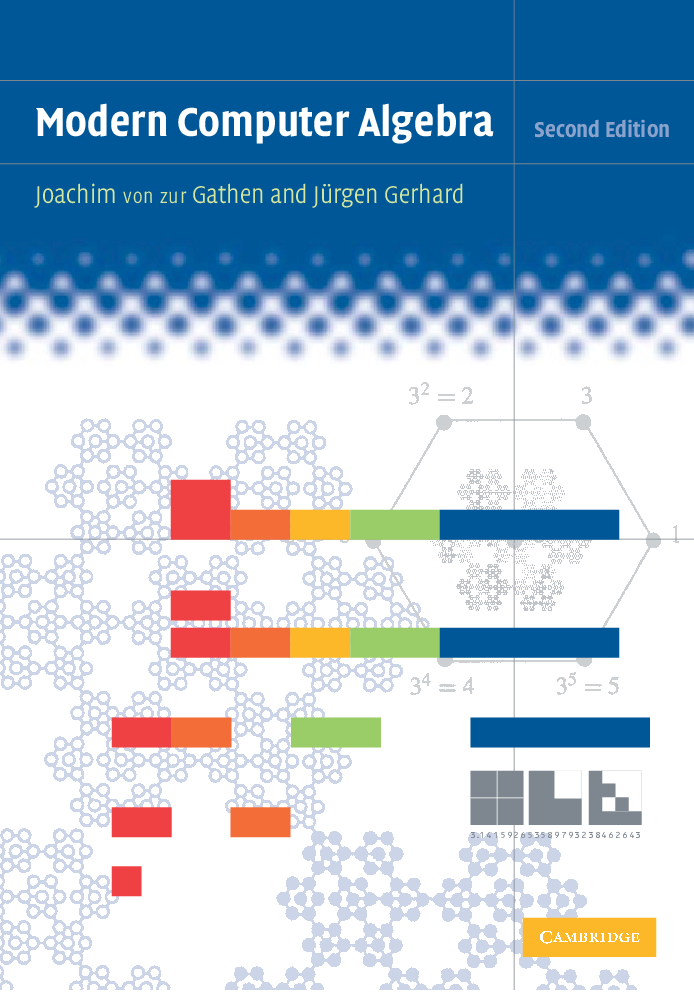
\includegraphics[width=0.8\textwidth]{modern.png}

        Dr. Jekyll is a computer algebraist
      \end{center}
    \end{column}
    \begin{column}{0.5\textwidth}
      \begin{center}
        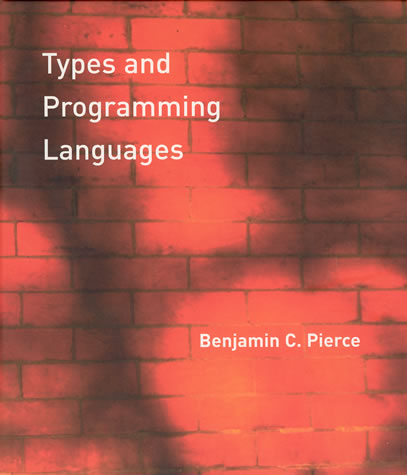
\includegraphics[width=0.8\textwidth]{types.jpg}
        
        Mr Type wastes precious research time reading about types and
        categorical semantics
      \end{center}
    \end{column}
  \end{columns}
\end{frame}

%%

\begin{pictureframe}
  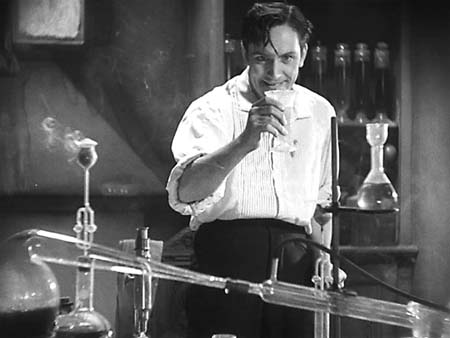
\includegraphics[width=\textwidth]{jekyll1}
\end{pictureframe}

%%
%%

\lstset{language=python}

\begin{frame}[fragile]
  \frametitle{Some trivialities}
  
  Suppose you have a computer program made \emph{exclusively} of
  ``steps'' in a given (Cartesian) category $\mathcal{C}$
  
  \begin{columns}
    \begin{column}{0.45\textwidth}
\begin{lstlisting}
  def foo(x in A,
          y in B):
    w = f(x, y)
    z = g(w, y)
    return z
\end{lstlisting}
    \end{column}
    \begin{column}{0.05\textwidth}
      \vfill
      \Large
      $\overset{F}{\Rightarrow}$
      \vfill
    \end{column}
    \begin{column}{0.5\textwidth}
\begin{lstlisting}
  def Ffoo(x in F(A),
           y in F(B)):
    w = F(f)(x, y)
    z = F(g)(w, y)
    return z
\end{lstlisting}
    \end{column}
  \end{columns}

  Then, a functor $F:\mathcal{C}\to\mathcal{D}$ permits us to
  translate programs \emph{working in $\mathcal{C}$} into programs
  \emph{working in $\mathcal{D}$}.

  \begin{figure}
    \centering
    \begin{tikzpicture}
      \newcommand{\noF}[1]{#1}
      \newcommand{\yesF}[1]{\ensuremath F(#1)}

      \foreach \x/\y in {noF/0cm,yesF/6.5cm} {
        \def\apF{\csname \x \endcsname}
        \begin{scope}[xshift=\y]
          \matrix[matrix of math nodes,column sep=1em,row sep=2em,ampersand replacement=\&]{
            \& |(B)| \apF{B}           \& |(CxB)| \apF{C\times B} \& |(D)| \apF{D} \\
            |(A)| \apF{A} \& |(AxB)| \apF{A\times B} \& |(C)| \apF{C}\\
          };
          \scriptsize
          \path[right hook->] (A) edge (AxB);
          \path[right hook->] (B) edge (AxB);
          \path[->] (AxB) edge node[auto]{$\apF{f}$} (C);
          \path[right hook->] (B) edge (CxB);
          \path[right hook->] (C) edge (CxB);
          \path[->] (CxB) edge node[auto]{$\apF{g}$} (D);
        \end{scope}
      }
    \end{tikzpicture}
  \end{figure}

  This \emph{principle} is most useful when the functor is an
  \emph{equivalence of categories}.
\end{frame}

%%

\begin{frame}[fragile]
  \frametitle{Some more trivialities}
  
  \begin{block}{}
    If we measure the computational complexity of a program by its
    number of \emph{elementary steps}, this measure is invariant under
    equivalence of categories, provided the equivalence functor sends
    \emph{elementary arrows} in $\mathcal{C}$ to \emph{elementary
      arrows} in $\mathcal{D}$.

    \begin{figure}
      \centering
      \begin{tikzpicture}
        \newcommand{\noF}[1]{#1}
        \newcommand{\yesF}[1]{\ensuremath F(#1)}
        \newcommand{\noar}{->}
        \newcommand{\yesar}{<-}

        \foreach \x/\y in {no/0cm,yes/6.5cm} {
          \def\apF{\csname \x F\endcsname}
          \def\apar{\csname \x ar\endcsname}

          \begin{scope}[xshift=\y]
            \matrix[matrix of math nodes,column sep=1em,row sep=2em,ampersand replacement=\&]{
              |(A)| \apF{A} \& |(B)| \apF{B} \& |(C)| \apF{C}\\
              \& |(D)| \apF{D} \& |(E)| \apF{E}\\
            };
            \scriptsize
            \path[\apar] (A) edge (B);
            \path[\apar] (B) edge (C);
            \path[\apar] (C) edge (E);
            \path[\apar,red] (A) edge (D);
            \path[\apar,red] (D) edge (E);
          \end{scope}
          \pause
        }
      \end{tikzpicture}
    \end{figure}

    \begin{uncoverenv}<2->
      And it also works with contravariant functors (dualities)!
    \end{uncoverenv}
  \end{block}  
  
  \begin{block}{}<3-> For most of this talk, we'll be interested in
    the category of \emph{vector spaces} and we will look at the
    \emph{transposition functor} (which is not exactly an
    equivalence). Thus you can forget everything about categories and
    just keep in mind that
    \[\trans{(AB)} = \trans{B}\trans{A}.\]
  \end{block}
\end{frame}

%%

\begin{pictureframe}
  
\includegraphics[width=\textwidth]{jekyll}
\end{pictureframe}


%%
%%

\begin{frame}
  \frametitle{Example: Middle product}

  \begin{block}{Newton iteration for the inverse of power series}
    \[G = 1/F \mod X^n, \qquad G + (1-GF)G = 1/F \mod X^{2n}.\]
    At each iteration,
    \[\deg G = n-1, \qquad \deg \left(F \bmod X^{2n}\right) = 2n-1, \qquad \deg GF = 3n-2,\]
    but \emph{$\quad X^n | (1-GF)\quad$} and \emph{$\quad\deg \left((1-GF)\bmod X^{2n}\right) = 2n-1$}.
  \end{block}
  
  \begin{equation*}
    GF = 
    \begin{pmatrix}
      g_0\\
      g_1 & g_0\\
      \hline
          & g_1 & g_0\\
          &     & g_1 & g_0\\
          \hline
          &     &     & g_1
    \end{pmatrix}
    \begin{pmatrix}
      f_0\\f_1\\f_2\\f_3
    \end{pmatrix}
    =
    \begin{pmatrix}
      1\\0\\\hline h_2\\h_3\\\hline h_4
    \end{pmatrix}
  \end{equation*}
\end{frame}

%%

\begin{frame}
  \frametitle{Example 1: Middle product}
  
  Set $\tilde{G} = X^nG(1/X) = g_0X^n + g_1X^{n-1} + \cdots + g_{n-1}X$, then
  \begin{equation*}
    \tilde{G}J =
    \begin{pmatrix}
      \\
      g_1\\
      g_0 & g_1\\
          & g_0
    \end{pmatrix}
    \begin{pmatrix}
      j_0\\j_1
    \end{pmatrix}
  \end{equation*}

  Hence \emph{$GF = X^n\trans{\tilde{G}}F  \bmod X^{2n}$}.

  \begin{block}{Complexity}
    \begin{itemize}
    \item The multiplication matrix of $\tilde{G}$ has $n^2$ non-zero
      coefficients: multiplying on the left or on the right costs
      $n^2$ multiplications plus $n(2n-1)$ additions by the row-column
      product. This is trivial and not very interesting.
    \item But we can compute $\tilde{G}J$ for any $J$ using only
      $\Mult(n)\in O(n\log n\loglog n)$ operations. The transposition
      principle says that we can compute $\trans{\tilde{G}}F$ for any
      $F$ using \emph{exactly} the same number of operations.
    \item On the other hand, computing $GF$ and then extracting the
      coefficients of the middle costs about $\Mult(2n)$
      operations. This is \emph{worse} by a factor of $2$!
    \end{itemize}
  \end{block}
\end{frame}

%% 

\begin{frame}
  \frametitle{Arithmetic circuits}

  \begin{block}{Algebraic complexity}
    \centering Fix a field $\K$. We construct circuits that evaluate
    arithmetic functions.
  \end{block}


  \begin{center}
    Three gates: Addition, duplication, multiplication by a fixed
    element $a\in\K$.
    
    \begin{tikzpicture}
      \tikzstyle{node}=[circle,thick,draw=black,minimum size=4mm]
      
      \begin{scope}
        \node(in1){};
        \node(nop1)[right of=in1]{};
        \node(in2)[right of=nop1]{};
        \node(nop2)[right of=in2]{};
        \node(in3)[right of=nop2]{};
        \node(nop3)[right of=in3]{};
        \node(in4)[right of=nop3]{};
        
        \node[node](plus)[below of=nop1]{$+$}
        edge(in1)
        edge(in2);
        \node(nop)[below of=nop2]{};
        \node[node](hub)[below of=in3]{$\hub$}
        edge(in3);
        \node[node](times)[below of=in4]{$*_a$}
        edge(in4);
        
        \node(out1)[below of=plus]{}
        edge(plus);
        \node(nop5)[right of=out1]{};
        \node(out2)[below of=nop]{}
        edge(hub);
        \node(nop6)[below of=hub]{};
        \node(out3)[right of=nop6]{}
        edge(hub);
        \node(out4)[below of=times]{}
        edge(times);
      \end{scope}
    \end{tikzpicture}
  \end{center}
\end{frame}

%%

\begin{frame}
  \frametitle{Arithmetic circuits}

  \begin{columns}
    \begin{column}{0.6\textwidth}
      \centering
      \begin{tikzpicture}
        \tikzstyle{node}=[circle,thick,draw=black,minimum size=4mm]
        
        \begin{scope}
          \node(x1){$x_1$};
          \node(x2)[right of=x1]{$x_2$};
          \node(x3)[right of=x2]{$x_3$};
          
          \node[node](d1)[below of=x2]{$\hub$}
          edge(x2);
          \node[node](d2)[below of=x3]{$\hub$}
          edge(x3);
          
          \node[node](p1)[below of=d1,xshift=-6mm]{$+$}
          edge(x1)
          edge(d1);
          \node[node](m1)[below of=d2]{$*_3$}
          edge(d2);
          
          \node[node](p2)[below of=p1]{$+$}
          edge(p1)
          edge(d2);
          \node[node](p3)[right of=p2]{$+$}
          edge(d1)
          edge(m1);
          
          \node(y1)[below of=p2]{$y_1$}
          edge(p2);
          \node(y2)[below of=p3]{$y_2$}
          edge(p3);
        \end{scope}
      \end{tikzpicture}
    \end{column}
    \begin{column}{0.4\textwidth}
      \begin{align*}
        y_1 &= x_1 + x_2 + x_3\\
        y_2 &= x_2 + 3x_3
      \end{align*}
      
      \Large
      \begin{gather*}
        \begin{pmatrix}
          1 & 1 & 1\\
          0 & 1 & 3
        \end{pmatrix}
      \end{gather*}
    \end{column}
  \end{columns}
\end{frame}

%%

\begin{frame}
  \frametitle{Transposition of an arithmetic circuit}

  \begin{columns}
    \begin{column}{0.6\textwidth}
      \centering
      \begin{tikzpicture}
        \tikzstyle{node}=[circle,thick,draw=black,minimum size=4mm]
        
        \begin{scope}
          \node(x1){$x_1$};
          \node(x2)[right of=x1]{$x_2$};
          \node(x3)[right of=x2]{$x_3$};
          
          \node[node](d1)[below of=x2]{$\hub$}
          edge(x2);
          \node[node](d2)[below of=x3]{$\hub$}
          edge(x3);
            
          \node[node](p1)[below of=d1,xshift=-6mm]{$+$}
          edge(x1)
          edge(d1);
          \node[node](m1)[below of=d2]{$*_3$}
          edge(d2);
          
          \node[node](p2)[below of=p1]{$+$}
          edge(p1)
          edge(d2);
          \node[node](p3)[right of=p2]{$+$}
          edge(d1)
          edge(m1);
          
          \node(y1)[below of=p2]{$y_1$}
          edge(p2);
          \node(y2)[below of=p3]{$y_2$}
          edge(p3);
        \end{scope}
        
        \begin{scope}[xshift=3.2cm, yshift=-0.23\textheight]
          \node(x){\Huge $\leftrightarrow$};
        \end{scope}
        
        \begin{scope}[xshift=4cm, yshift=-0.425\textheight]
          \node(x1){$x_1'$};
          \node(x2)[right of=x1]{$x_2'$};
          \node(x3)[right of=x2]{$x_3'$};
          
          \node[node](d1)[above of=x2]{\alt<2>{$+$}{$\hub$}}
          edge(x2);
          \node[node](d2)[above of=x3]{\alt<2>{$+$}{$\hub$}}
          edge(x3);
          
          \node[node](p1)[above of=d1,xshift=-5mm]{\alt<2>{$\hub$}{$+$}}
          edge(x1)
          edge(d1);
          \node[node](m1)[above of=d2]{$*_3$}
          edge(d2);
          
          \node[node](p2)[above of=p1]{\alt<2>{$\hub$}{$+$}}
          edge(p1)
          edge(d2);
          \node[node](p3)[right of=p2]{\alt<2>{$\hub$}{$+$}}
          edge(d1)
          edge(m1);
          
          \node(y1)[above of=p2]{$y_1'$}
          edge(p2);
          \node(y2)[above of=p3]{$y_2'$}
          edge(p3);
        \end{scope}
      \end{tikzpicture}
    \end{column}
    \begin{column}{0.4\textwidth}
      \begin{align*}
        y_1 &= x_1 + x_2 + x_3\\
        y_2 &= x_2 + 3x_3
      \end{align*}
      
      \Large
      \begin{gather*}
        \begin{pmatrix}
          1 & 1 & 1\\
          0 & 1 & 3
        \end{pmatrix}\\
        \updownarrow\\
        \begin{pmatrix}
          1 & 0\\
          1 & 1\\
          1 & 3\\
        \end{pmatrix}
      \end{gather*}
    \end{column}
  \end{columns}
\end{frame}

%%

\begin{frame}
  \frametitle{Arithmetic Circuits: uniform vs. non-uniform}

  \begin{definition}[Circuit family]
    A \emph{circuit family} is a family $(C_0,C_1,\ldots)$ of circuits
    indexed by $\N$ such that $C_n$ has $n$ inputs.
  \end{definition}
  
  \begin{itemize}
  \item This gives the usual notion of complexity as a mapping
    $\N\to\N$.
  \item \alert{Any Turing-undecidable problem has a trivial
      \emph{polynomial-size} circuit family deciding it.}
  \end{itemize}

  \begin{definition}[Uniform circuit family]
    A circuit family $(C_0,C_1,\ldots)$ is said to be \emph{uniform}
    if there is a $\log n$-space bounded touring machine which on
    input $1^n$ outputs a representation of $C_n$.
  \end{definition}

  \begin{itemize}
  \item The transposition principle preserves uniformity.
  \item However, notice that there is no consistent way of analysing
    \emph{space complexity} in this model.
  \end{itemize}
\end{frame}

%%

\begin{frame}
  \frametitle{Vandermonde matrices}

  Let $P$ be a degree $n$ polynomial and let $a_1,\ldots,a_m$ be
  evaluation points, then
  \begin{equation*}
    V_{a_1,\ldots,a_m}P =
    \begin{pmatrix}
      1 & a_1 & \cdots & a_1^n\\
      \vdots & \vdots & & \vdots\\
      1 & a_m & \cdots & a_m^n
    \end{pmatrix}
    \begin{pmatrix}
      p_0\\p_1\\\vdots\\p_n
    \end{pmatrix}
    =
    \begin{pmatrix}
      P(a_1)\\\vdots\\P(a_m)
    \end{pmatrix}
  \end{equation*}
  where $V_{a_1,\ldots,a_m}$ is a Vandermonde matrix, the transposed
  problem is known as \emph{weighted Newton sums}.

  \begin{block}{Applications of the transposition principle}
    \begin{itemize}
    \item Solving sparse polynomial systems
      \parencite{canny+kaltofen+yagati89};
    \item Improving the complexity of multipoint evaluation;
    \item Equivalence between the complexities of interpolation and
      multipoint evaluation \parencite{bostan+schost04}.
    \end{itemize}
  \end{block}
\end{frame}

%%

{\setbeamertemplate{frametitle continuation}{}
\begin{frame}[allowframebreaks]
  \frametitle{Transposed modular multiplication}

  \begin{block}{Modular reduction}
    Fix $f\in\K[X]$ of degree $n+1$, let
    \begin{equation*}
      \begin{aligned}
        \bmod_f:\K[X]&\to\K[X]_n,\\
        a&\mapsto a\bmod f.
      \end{aligned}
    \end{equation*}
  \end{block}
  
  \begin{block}{Identifying dual spaces with power series}
    Identify $\dual{(\K[X])}$ to $\K[[1/X]]$ via
    \begin{equation*}
      \braket{\alpha}{b} = [\alpha b]_0
      \qquad\text{for $\alpha\in\K[[1/X]], b\in\K[X]$,}
    \end{equation*}
    and similarly identify $\dual{(\K[X]_n)}$ to $\K[1/X]_n$.
  \end{block}
  
  \begin{theorem}[Transposed $\bmod$ = extension of linear recurrences]
    Denote by $\dual{\bmod_f}:\K[1/X]_n\to\K[[1/X]]$ the dual map to
    $\bmod_f$, then 
    \begin{equation*}
      \braket{\dual{\bmod_f}(\alpha)}{X^if} = 
      \braket{\alpha}{X^if\bmod f} = 0
      \qquad\text{for any $i\ge0$.}
    \end{equation*}

    Set $\beta=\dual{\bmod_f}(\alpha)$, then
    \begin{equation*}
      \braket{\beta}{X^if} = [X^i\beta f]_0 = \sum_{j=0}^{n+1}\beta_{j+i}f_j = 0
      \qquad\text{for any $i\ge0$,}
    \end{equation*}
    thus the coefficients of $\beta$ satisfy a linear recurrence with
    characteristic polynomial $f$ and the initial conditions are given by
    \begin{equation*}
      \beta_i = \braket{\beta}{X^i} = \braket{\alpha}{X^i\bmod f} = \braket{\alpha}{X^i} = \alpha_i
      \qquad\text{for $i\le n$.}
    \end{equation*}
  \end{theorem}

  \begin{block}{Applications of the transposition principle}
    \begin{itemize}
    \item Fastest algorithm to develop the Fibonacci sequence (and any other LRSCC);
    \item Middle product + $\dual{\bmod_f}$ = transposed multiplication in $\K[X]/f(X)$;
    \item Easy generalization to higher dimension (for example,
      \cite{pascal+schost06} treat the case of $\K[X,Y]/I$ with $I$ a
      triangular ideal).
    \end{itemize}
  \end{block}
\end{frame}
}
%%

\begin{frame}
  \frametitle{Polynomial evaluation}

  \begin{block}{Power projection}
    Let $A$ be a $\K$-algebra. Fix $\sigma\in A$ and consider the
    \emph{polynomial evaluation morphism}
    \begin{equation*}
      \begin{aligned}
        \ev_\sigma:\K[X]&\to A,\\
        f &\mapsto f(\sigma).
      \end{aligned}
    \end{equation*}
    
    Identify $\dual{(\K[X])}$ with $\K[[1/X]]$, then
    \begin{equation*}
      \begin{aligned}
        \dual{\ev_\sigma}:\dual{A}&\to\K[[1/X]],\\
        \ell &\mapsto \sum_{i\ge0}\frac{\ell(\sigma^i)}{X^i}
      \end{aligned}
    \end{equation*}
    is called \emph{power projection} (denoted by $\proj_\sigma$).
  \end{block}
\end{frame}

%%

\begin{frame}
  \frametitle{Polynomial evaluation: applications}

  \begin{block}{Minimal polynomials \cite{shoup94,shoup99}}
    Let $A$ be $n$-dimensional. To compute the minimal polynomial
    of $\sigma$, repeat the following steps:
    \begin{itemize}
    \item pick up a random form $\ell\in\dual{A}$,
    \item compute $\left(\ell(1), \ell(\sigma), \ldots,
        \ell(\sigma^{2n-1})\right)$ using \emph{transposed polynomial
        evaluation},
    \item find a factor of $\pi_\sigma$ using the Berlekamp-Massey
      algorithm.
    \end{itemize}
  \end{block}

  \begin{block}{Complexity}
    The complexity is usually dominated by the polynomial evaluation step:
    \begin{itemize}
    \item $2n-1$ products in $A$ using Horner's rule $\;\Rightarrow
      O(n^2)$ at best.
    \item In the case $A=\K[X]/(f)$ or $A=\K[X]/(f,g)$, transposing
      \emph{modular composition} yields
      $O\left(n^{(\omega+1)/2}\right)$, or even
      $O\left(n^{1+o(1)}\right)$ by \parencite{kedlaya+umans08}.
    \end{itemize}
  \end{block}
\end{frame}

%%

\begin{frame}[fragile]
  \frametitle{Automatic differentiation}
  
  \textbf{Problem:} We have a computer program that computes an
  unknown function $f:\R^n\to\R^m$, we want to evaluate the Jacobian
  matrix of $f$ at a point $P\in R^n$.

  \begin{columns}
    \begin{column}{0.5\textwidth}
      \begin{figure}
        \centering
        \begin{tikzpicture}
          \tikzstyle{node}=[circle,thick,draw=black,minimum size=4mm]
          \tikzstyle{arg}=[rectangle,thin,draw=black,minimum size=4mm]
          
          \begin{scope}
            \node[arg](in1){$x_1$};
            \node[arg,right of=in1](in2){$x_2$};
            \node[arg,right of=in2](in3){$x_3$};
            \node[node,below of=in1,xshift=5mm](times1){$*$};
            \node[node,below of=times1,xshift=5mm](times2){$*$};
            \node[arg,below of=times2](out){$y_1$};

            \path[->]
            (in1) edge (times1)
            (in2) edge (times1)
            (times1) edge (times2)
            (in3) edge (times2)
            (times2) edge (out);
          \end{scope}
        \end{tikzpicture}
      \end{figure}  
    \end{column}
    \begin{column}{0.5\textwidth}
      \centering
\begin{lstlisting}
def f(x1, x2, x3):
  t = x1 * x2
  y1 = t * x3
  return y1
\end{lstlisting}
    \end{column}
  \end{columns}
\end{frame}

%%

\begin{frame}[fragile]
  \frametitle{Automatic differentiation}

  Construct a \emph{linearization} of the circuit by substituting each
  node with its Jacobian at $P$.
  
  \begin{columns}
    \begin{column}{0.5\textwidth}
      \begin{figure}
        \centering
        \begin{tikzpicture}
          \tikzstyle{node}=[circle,thick,draw=black,minimum size=4mm]
          \tikzstyle{arg}=[rectangle,thin,draw=black,minimum size=4mm]
          
          \begin{scope}[node distance=1.3cm]
            \node[arg](in1){$\diff x_1$};
            \node[arg,right of=in1](in2){$\diff x_2$};
            \node[arg,right of=in2](in3){$\diff x_3$};
            \node[node,below of=in1,xshift=5mm](times1){\small$(b,a)$};
            \node[node,below of=times1,xshift=5mm](times2){\small$(c,ab)$};
            \node[arg,below of=times2](out){$\diff y_1$};

            \path[->]
            (in1) edge (times1)
            (in2) edge (times1)
            (times1) edge (times2)
            (in3) edge (times2)
            (times2) edge (out);
          \end{scope}
        \end{tikzpicture}
      \end{figure}
    \end{column}
    \begin{column}{0.5\textwidth}
      \centering
\begin{lstlisting}
def df(dx1, dx2, dx3):
  dt = b*dx1 + a*dx2
  dy1 = c*dt + a*b*dx3
  return dy1
\end{lstlisting}
    \end{column}
  \end{columns}

  \bigskip

  In the example we have chosen to linearize at the point $P=(a,b,c)$.
\end{frame}

%%

\begin{frame}[fragile]
  \frametitle{Automatic differentiation}

  Now to compute the Jacobian matrix, successively evaluating the
  linearized function at $\diff x_1$, $\diff x_2$ and $\diff x_3$
  gives
  \[\nabla_{(a,b,c)}f = (bc, ac, ab).\]

  
  \begin{columns}
    \begin{column}{0.5\textwidth}
      \begin{figure}
        \centering
        \begin{tikzpicture}
          \tikzstyle{node}=[circle,thick,draw=black,minimum size=4mm]
          \tikzstyle{arg}=[rectangle,thin,draw=black,minimum size=4mm]
          
          \begin{scope}[node distance=1.3cm]
            \node[arg](in1){$\diff x_1$};
            \node[arg,right of=in1](in2){$\diff x_2$};
            \node[arg,right of=in2](in3){$\diff x_3$};
            \node[node,below of=in1,xshift=5mm](times1){\small$(b,a)$};
            \node[node,below of=times1,xshift=5mm](times2){\small$(c,ab)$};
            \node[arg,below of=times2](out){$\diff y_1$};

            \begin{altenv}<2>
              {\path[<-]}{}{\path[->]}{}
              (in1) edge (times1)
              (in2) edge (times1)
              (times1) edge (times2)
              (in3) edge (times2)
              (times2) edge (out);
            \end{altenv}
          \end{scope}
        \end{tikzpicture}
      \end{figure}
    \end{column}
    \begin{column}{0.5\textwidth}
      \centering
      \begin{onlyenv}<1>
\begin{lstlisting}
def df(dx1, dx2, dx3):
  dt = b*dx1 + a*dx2
  dy1 = c*dt + a*b*dx3
  return dy1
\end{lstlisting}
      \end{onlyenv}
      \begin{onlyenv}<2>
\begin{lstlisting}
def df(dy1):
  dt = c*dy1
  dx3 = a*b*dy1
  dx1 = b*dt
  dx2 = a*dt
  return dx1, dx2, dx3
\end{lstlisting}
      \end{onlyenv}
    \end{column}
  \end{columns}

  \bigskip

  \begin{uncoverenv}<2> Alternatively, transposing and evaluating at
    $\diff y_1$ \emph{directly} yields the same result.
  \end{uncoverenv}
\end{frame}


%% 
%%

\begin{pictureframe}
  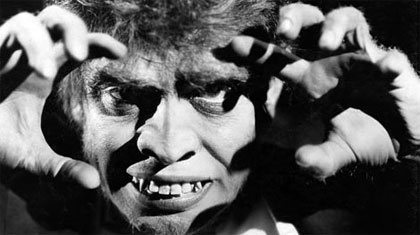
\includegraphics[width=\textwidth]{hyde2}
\end{pictureframe}

%%

\begin{frame}[fragile]
  \tiny
  \frametitle{Why \emph{automatic} transposition?}

  \begin{columns}
    \begin{column}{0.5\textwidth}
      \begin{center}
        \begin{minipage}{\textwidth}
\begin{verbatim}
void reduc_doit(GF2X& A0, GF2X& A1, const GF2X& A,
	long init, long d, bool plusone){
  if (d <= 2){
    A0 = GF2X(0, coeff(A,init));
    A1 = GF2X(0, coeff(A,init+1));
    return;
  }
   
  long dp = d/2;
  GF2X A10, A11;

  reduc_doit(A0, A1, A, init, dp, plusone);
  reduc_doit(A10, A11, A, init+dp, dp, plusone);
 
  ShiftAdd(A0, A11, 1);
  if (plusone) A0 += A11;
  A1 += A10 + A11;

  long i = 1;
  bool even = true;
  while (2*i != d){
    ShiftAdd(A0, A10, i);
    ShiftAdd(A1, A11, i);
    i = 2*i;
    even = !even;
  }
  
  if (plusone && !even) {
    A0 += A10;
    A1 += A11;
  }
}
\end{verbatim}
        \end{minipage}
      \end{center}
    \end{column}

    \begin{column}{0.5\textwidth}
      \begin{center}
        \begin{minipage}{\textwidth}
\begin{verbatim}
void treduc_doit(GF2X& A, const GF2X& A0, const GF2X& A1, long d,
	bool plusone){
  if (d <= 2){
    SetCoeff(A, 0, coeff(A0, 0));
    SetCoeff(A, 1, coeff(A1, 0));
    return;
  }
   
  long dp = d/2;
  long hdp = dp/2;

  GF2X A00, A01, A10, A11;
  A00 = trunc(A0, hdp);
  A01 = trunc(A1, hdp);

  A10 = A01;
  if (plusone) A11 = A00;
  else A11 = 0;
  A11 += A01 + RightShift(trunc(A0, hdp+1), 1);
  long i = 1;
  bool even = true;
  while (2*i != d){
    A10 += RightShift(trunc(A0, hdp+i), i);
    A11 += RightShift(trunc(A1, hdp+i), i);
    i = 2*i;
    even = !even;
  }
  
  if (plusone && !even) {
    A10 += trunc(A0, hdp);
    A11 += trunc(A1, hdp);
  }
  
  GF2X B0, B1;
  treduc_doit(B0, A00, A01, dp, plusone);
  treduc_doit(B1, A10, A11, dp, plusone);
  A = B0 + LeftShift(B1,dp);
}
\end{verbatim}
        \end{minipage}
      \end{center}
    \end{column}
    \end{columns}
\end{frame}

%%

\begin{frame}
  \frametitle{Why \emph{automatic} transposition?}

  Pioneered by \cite{bostan+lecerf+schost:tellegen}, who automatically
  transpose a very restricted language

  \begin{block}{Why?}
    \begin{itemize}
    \item Algorithms are hard to transpose, transposed algorithms are
      hard or impossible to understand;
    \item How to be confident that a transposed algorithm is well
      implemented if no one understands it?
    \item When proving programs with a proof assistant, why should we do
      the work twice?
    \end{itemize}
  \end{block}
  
  \begin{block}{Problems}
    \begin{itemize}
    \item We often want to transpose \emph{multilinear} algorithms
      (e.g., polynomial multiplication).
    \item We want linear algorithms to be parametrized by algebraic
      arguments (e.g., modular reduction).
    \item Programming languages are not designed to reason about
      computations in categories other than $\mathbf{Set}$.
    \end{itemize}
  \end{block}
\end{frame}

%%

\begin{frame}
  \frametitle{Multilinearity}

  \begin{center}
    \begin{tikzpicture}
      \tikzstyle{node}=[circle,thick,draw=black,minimum size=4mm]
      \tikzstyle{arg}=[rectangle,thin,draw=black,minimum size=4mm]
      \tikzstyle{nodeg}=[circle,thick,draw=gray,minimum size=4mm]
      \tikzstyle{argg}=[rectangle,thin,draw=gray,minimum size=4mm]
      
      \begin{scope}
        \node[arg](in1){$x_1$};
        \node[arg,right of=in1](in2){$x_2$};
        \node[arg,right of=in2](in3){$x_3$};
        \node[node,below of=in1,xshift=5mm](times1){$*$};
        \node[node,below of=times1,xshift=5mm](times2){$*$};
        \node[arg,below of=times2](out){$y_1$};
        
        \path[->]
        (in1) edge (times1)
        (in2) edge (times1)
        (times1) edge (times2)
        (in3) edge (times2)
        (times2) edge (out);
      \end{scope}
      
      \begin{scope}[xshift=4cm]
        \node[argg](in1){\color{gray}{$x_1$}};
        \node[arg,right of=in1](in2){$x_2$};
        \node[argg,right of=in2](in3){\color{gray}{$x_3$}};
        \node[node,below of=in1,xshift=5mm](times1){$*_{x_1}$};
        \node[node,below of=times1,xshift=5mm](times2){$*_{x_3}$};
        \node[arg,below of=times2](out){$y_1$};
        
        \path[->]
        (in2) edge (times1)
        (times1) edge (times2)
        (times2) edge (out);
        
        \path[->,draw=gray,dashed]
        (in1) edge (times1)
        (in3) edge (times2);
      \end{scope}
      
      \begin{scope}[xshift=8cm]
        \node[arg](in1){$x_3$};
        \node[arg,right of=in1](in2){$y_1^\ast$};
        \node[arg,right of=in2](in3){$x_1$};
        \node[node,below of=in1,xshift=5mm](times1){$*$};
        \node[node,below of=times1,xshift=5mm](times2){$*$};
        \node[arg,below of=times2](out){$x_2^\ast$};

        \path[->]
        (in2) edge (times1)
        (times1) edge (times2)
        (times2) edge (out)
        (in3) edge (times2)
        (in1) edge (times1);
      \end{scope}
    \end{tikzpicture}  
  \end{center}

  \begin{itemize}
  \item Almost anytime we want to transpose, we end-up
    \emph{linearising} a circuit with multiplication nodes.
  \item Other constructs such as \texttt{if} statements and
    \texttt{for} loops need to be linearised too.
  \item Can we automatically deduce any possible linearisation of a
    program?
  \item \alert{Type inference systems can help us}
  \end{itemize}
\end{frame}

%%

\begin{frame}[fragile]
  \frametitle{Linearity inference}

  \begin{center}
    Suppose given a type \lstinline{R} implementing a ring. We want to
    define types \alert{\lstinline{L}} (for \emph{linear}) and
    \alert{\lstinline{S}} (for \emph{scalar}) such that the following
      equations hold
  \end{center}
  
  \begin{columns}
    \begin{column}{0.5\textwidth}
  \begin{semiverbatim}
    plus :: L -> L -> L
    plus :: S -> S -> S
  \end{semiverbatim}
    \end{column}
    \begin{column}{0.5\textwidth}
      \uncover<2>{\[\forall
        \alpha\in\{L,S\}.\alpha\ra\alpha\ra\alpha\]}
    \end{column}
  \end{columns}
  
  \begin{columns}[c]
    \begin{column}{0.5\textwidth}
  \begin{semiverbatim}
    times :: L -> S -> L
    \alt<2>{\st{times :: S {} -> L {} -> L}}{times :: S -> L -> L}
    times :: S -> S -> S
  \end{semiverbatim}
    \end{column}
    \begin{column}{0.5\textwidth}
      \uncover<2>{\[\forall
        \alpha\in\{L,S\}.\alpha\ra S\ra\alpha\]}
    \end{column}
  \end{columns}

  \begin{columns}
    \begin{column}{0.5\textwidth}
  \begin{semiverbatim}
    zero :: L
    zero :: S
  \end{semiverbatim}
    \end{column}
    \begin{column}{0.5\textwidth}
      \uncover<2>{\[\forall
        \alpha\in\{L,S\}.\alpha\]}      
    \end{column}
  \end{columns}

  \begin{columns}
    \begin{column}{0.5\textwidth}
  \begin{semiverbatim}
    one :: S
  \end{semiverbatim}
    \end{column}
    \begin{column}{0.5\textwidth}
    \end{column}
  \end{columns}
\end{frame}  

%%

\begin{frame}[fragile]
  \frametitle{Linearity inference}
  
  \begin{center}
    The solution in Haskell
  \end{center}

  \begin{lstlisting}
    data L = L R
    data S = S R
    
    class Ring r where
      zero :: r
      (<+>) :: r -> r -> r
      neg :: r -> r
      (<*>) :: r -> S -> r

    one = S oneR
    (S a) == (S b) = a == b
  \end{lstlisting}

  \begin{center}
    To treat \alert{\lstinline{times :: S -> L -> L}}, we extend the
    Hindley-Milner type inference to handle lists of acceptable
    unifications.
  \end{center}
\end{frame}

%%

\begin{frame}
  \frametitle{Algebraic parameters}

  \begin{itemize}
  \item Once a program has been linearized, all the scalar values
    \emph{must be precomputed} in order to generate the corresponding
    arithmetic circuit;
  \item This reflects the fact that arithmetic circuits do not model
    \emph{space complexity};
  \item While this \emph{potentially increases the storage needed},
    it is seldom a problem for real-world algorithms.
  \item Our language \texttt{transalpyne} automatically handles
    multilinearity and algebraic parameters to generate transposed
    code: \url{http://transalpyne.gforge.inria.fr}.
  \end{itemize}
\end{frame}

\begin{frame}{Better idioms?}
  \begin{itemize}
  \item Functional languages implicitly work in the category $\mathbf{Set}$;
  \item Some advanced ones (e.g., Haskell with \emph{arrows}) permit
    to reflect some (very small) subcategory of $\mathbf{Set}$ in
    their type system;
  \item By adding some expressiveness to these languages, it should
    be possible to program in a style close to that of arithmetic
    circuits, while devoiding the programs from any link to a
    concrete category. Ultimately this leads to
    \emph{self-transposing programs}. (Some experiments already
    worked in Haskell, now studying Agda)
  \end{itemize}
\end{frame}

%%
%%

{
  \setbeamertemplate{navigation symbols}{}
  \setbeamertemplate{background canvas}{
\includegraphics[width=\paperwidth]{hyde}}
  \begin{frame}[plain]
    \vspace{8cm}
    \begin{center}
      \textcolor{white}{\Huge The End?}
    \end{center}
  \end{frame}
}

%%

{\setbeamertemplate{navigation symbols}{}
\begin{frame}[allowframebreaks]
  \frametitle{References}
  
  \printbibliography
\end{frame}
}

%%
%%

\end{document}




%%% Local Variables: 
%%% mode:flyspell
%%% ispell-local-dictionary:"american"
%%% mode: TeX-PDF
%%% mode: reftex
%%% TeX-master: t
%%% End: 
%
% LocalWords:  Tellegen
